\section{Date: 2024-12-13}
\noindent \textbf{Series ID: CPACPOP} 

\noindent This series is titled Resident Population in the Pacific Census Division and has a frequency of Annual. The units are Thousands of Persons and the seasonal adjustment is Not Seasonally Adjusted.The observation start date is 1900-01-01 and the observation end date is 2023-01-01.The popularity of this series is 2. \\ 

\noindent \textbf{Series ID: A371RD3Q086SBEA} 

\noindent This series is titled Private inventories (implicit price deflator) and has a frequency of Quarterly. The units are Index 2017=100 and the seasonal adjustment is Seasonally Adjusted.The observation start date is 1947-01-01 and the observation end date is 2024-07-01.The popularity of this series is 1. \\ 

\subsection{Regression Tables and Plots}
\begin{center}
\begin{tabular}{lclc}
\toprule
\textbf{Dep. Variable:}       & value\_fred\_A371RD3Q086SBEA & \textbf{  R-squared:         } &     0.926   \\
\textbf{Model:}               &             OLS              & \textbf{  Adj. R-squared:    } &     0.925   \\
\textbf{Method:}              &        Least Squares         & \textbf{  F-statistic:       } &     943.3   \\
\textbf{Date:}                &       Fri, 13 Dec 2024       & \textbf{  Prob (F-statistic):} &  3.16e-44   \\
\textbf{Time:}                &           11:39:24           & \textbf{  Log-Likelihood:    } &   -274.41   \\
\textbf{No. Observations:}    &                77            & \textbf{  AIC:               } &     552.8   \\
\textbf{Df Residuals:}        &                75            & \textbf{  BIC:               } &     557.5   \\
\textbf{Df Model:}            &                 1            & \textbf{                     } &             \\
\textbf{Covariance Type:}     &          nonrobust           & \textbf{                     } &             \\
\bottomrule
\end{tabular}
\begin{tabular}{lcccccc}
                              & \textbf{coef} & \textbf{std err} & \textbf{t} & \textbf{P$> |$t$|$} & \textbf{[0.025} & \textbf{0.975]}  \\
\midrule
\textbf{const}                &     -26.4468  &        2.936     &    -9.007  &         0.000        &      -32.296    &      -20.597     \\
\textbf{value\_fred\_CPACPOP} &       0.0024  &     7.83e-05     &    30.713  &         0.000        &        0.002    &        0.003     \\
\bottomrule
\end{tabular}
\begin{tabular}{lclc}
\textbf{Omnibus:}       & 10.077 & \textbf{  Durbin-Watson:     } &    0.170  \\
\textbf{Prob(Omnibus):} &  0.006 & \textbf{  Jarque-Bera (JB):  } &   10.038  \\
\textbf{Skew:}          &  0.763 & \textbf{  Prob(JB):          } &  0.00661  \\
\textbf{Kurtosis:}      &  3.895 & \textbf{  Cond. No.          } & 1.12e+05  \\
\bottomrule
\end{tabular}
%\caption{OLS Regression Results}
\end{center}

Notes: \newline
 [1] Standard Errors assume that the covariance matrix of the errors is correctly specified. \newline
 [2] The condition number is large, 1.12e+05. This might indicate that there are \newline
 strong multicollinearity or other numerical problems.

\begin{figure}
\centering
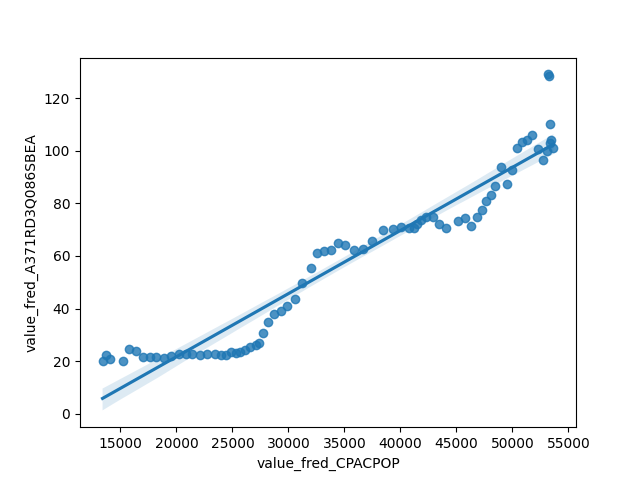
\includegraphics[scale = 0.9]{plots/plot_2024-12-13.png}
\caption{Regression Plot for 2024-12-13}
\end{figure}
\newpage
